\frameT{Preference Trees}{
	\begin{itemize}
		\item Let $\cI$ be a set of binary issues. The \tbf{combinatorial domain}
					$\CD(\cI)$ is the set of \tit{outcomes} represented by
					complete and consistent sets of literals over $\cI$.
		\item A \tbf{P-tree} $T$ over $\CD(\cI)$
					is a binary tree whose nodes, other than the leaves, are labeled with
					propositional formulas over $\cI$.
		\item Given an outcome $M \in \CD(\cI)$, the \tbf{leaf} $l_T(M)$
					is the leaf reached by traversing the tree $T$ according to $M$.
					When at a node $N$ labeled with $\varphi$, if $M\models \varphi$,
					we descend to the left child of $N$; otherwise, to the right.
		\item For $M, M'\in \CD(\cI)$, we have $M\succ_T M'$ if $l_T(M) \succ_T l_T(M')$,
					and $M \approx_T M'$ if $l_T(M)=l_T(M')$. Outcome $M$ is \tbf{optimal} if 
					there exists no $M'$ such that $M' \succ_T M$.
	\end{itemize}
}

\frameT{Compact Representation of P-trees}{
	A \tit{compact P-tree} over $\CD(\cI)$ is a tree where
	\begin{enumerate}
		\setlength\itemsep{0em}
		\item every node is labeled with a Boolean formula over $\cI$, and
	  \item every non-leaf node $t$ labeled with $\varphi$ has either
	        two outgoing edges (Figure (a)), or one 
	    		outgoing edge pointing left (Figure (b)),
					right (Figure (c)), or straight-down (Figure (d)).
	\end{enumerate}
	
	\begin{figure}[ht!]
	  \centering
	    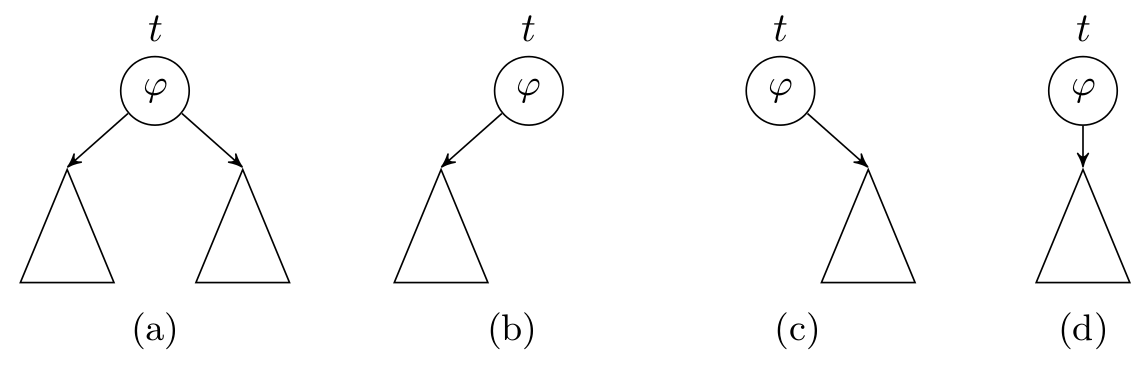
\includegraphics[width=0.9\textwidth]{figs/PTrees/ptrees.png}
	  \caption{Compact P-trees}
	\end{figure}
}

\frameT{Relative Expressivity of Preference Languages}{
	\begin{center}
		Poss-theories = ASO-rules $\subsetsim$ 
			\dual{LP-trees/\dual{$\cap$/\dual{PLP-trees/\dual{$\cap$/P-trees}}}}
			$\subset$ ASO-theories
	\end{center}
}

\frameT{Computational Complexity Results}{
	{\sc DomTest}: is it that $o \succeq_T o'$ in P-tree $T$?\\
	{\sc OptTest}: is outcome $o$ optimal w.r.t $T$?\\
	{\sc OptProp}: is there an optimal outcome $o$ w.r.t $T$ st $o \models \alpha$?
	
	\begin{figure}
		\centering

	  \begin{tabular}[0.5\textwidth]{ | c | c | c | c | }
	    \hline
	     & {\sc DomTest}& {\sc OptTest} & {\sc OptProp} \\
			\hline
			LP-tree & P & P & P \\
			\hline
			\pbox{20cm}{ASO-rule/ \\ Poss-theory} & P & coNP-c & $\deltap{2}$($P^{NP}$) \\
	    \hline
	    \tbf{P-tree} & \tbf{P} & \tbf{coNP-c}\fn{The complement problem is reduced from the SAT problem.}
				& \tbf{$\deltap{2}$($P^{NP}$)-c}\fn{The problem is reduced from the Maximum Satisfying 
																					Assignment (MSA) problem.}\\
			\hline
			ASO-theory & P & coNP-c & $\sigmap{2}$($NP^{NP}$)-c \\
	    \hline
			%ACP-net & NP-hard & P & P \\
	    %\hline
			%CCP-net & PSPACE-c & PSPACE-c? & PSPACE-c? \\
	    %\hline
	  \end{tabular}

		\caption{Computational complexity results}

	\end{figure}
}

\frameT{Partial Lexicographic Preference Trees (PLP-Tree)}{
	A \tit{PLP-tree} over $\CD(\cI)$ is a labeled tree, where
	\begin{enumerate}
		\setlength\itemsep{0em}
		\item every node $t$ is labeled with a attribute $\Attr(t)$ in $\cI$ and
					a conditional preference table $\CPT(t)$,
	  \item every non-leaf node $t$ has either one unlabeled outgoing edge or multiple
					outgoing edges labeled, each labeled by some value in $\Dom(\Attr(t))$, and
		\item every attribute appears \tit{at most} once on every branch.
	\end{enumerate}
}

\frameT{Partial Lexicographic Preference Trees (PLP-Tree)}{
	\begin{figure}[ht!]
	  \centering
	    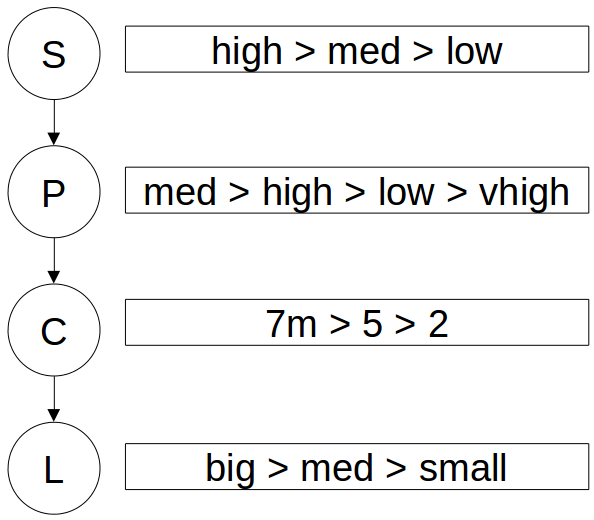
\includegraphics[width=0.4\textwidth]{figs/Cars/uiuptree.png}
	  \caption{A UIUP PLP-tree}
	\end{figure}

	According to this UIUP PLP-tree, \tit{Car1} is preferred to \tit{Car2}.
}

\frameT{Partial Lexicographic Preference Trees (PLP-Tree)}{
	\begin{figure}[ht!]
	  \centering
	    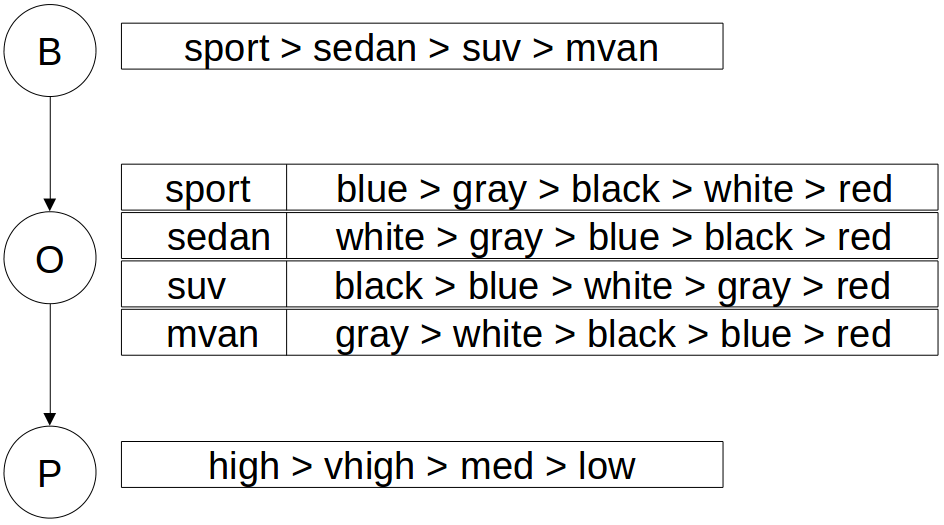
\includegraphics[width=0.65\textwidth]{figs/Cars/uicptree.png}
	  \caption{A UICP PLP-tree}
	\end{figure}

	According to this UICP PLP-tree, \tit{Car2} is preferred to \tit{Car1}.
}

\frameT{Partial Lexicographic Preference Trees (PLP-Tree)}{
	\begin{figure}[ht!]
	  \centering
	    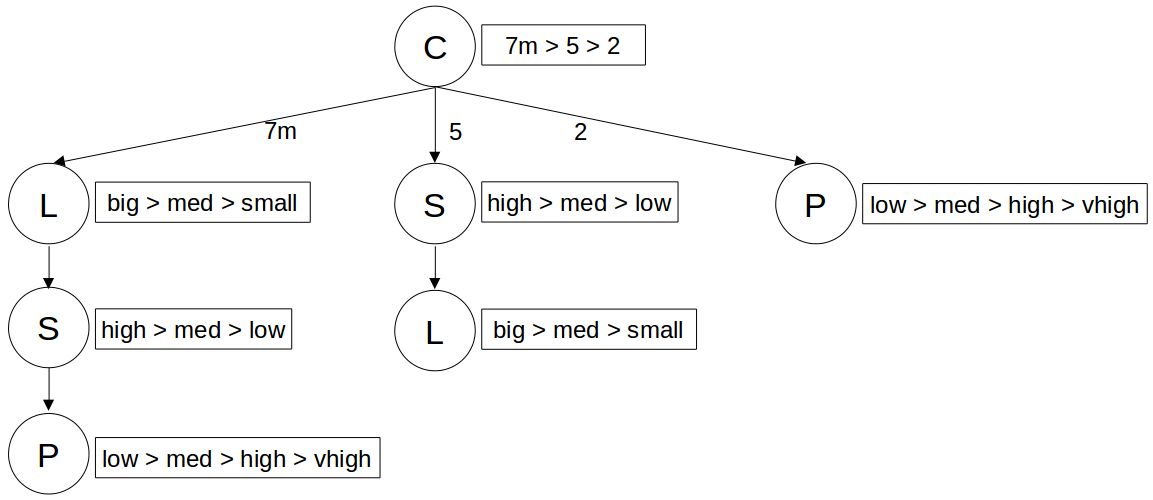
\includegraphics[width=0.9\textwidth]{figs/Cars/ciuptree.png}
	  \caption{A CIUP PLP-tree}
	\end{figure}

	According to this CICP PLP-tree, \tit{Car1} is preferred to \tit{Car2}.
}

\frameT{Partial Lexicographic Preference Trees (PLP-Tree)}{
	\begin{figure}[ht!]
	  \centering
	    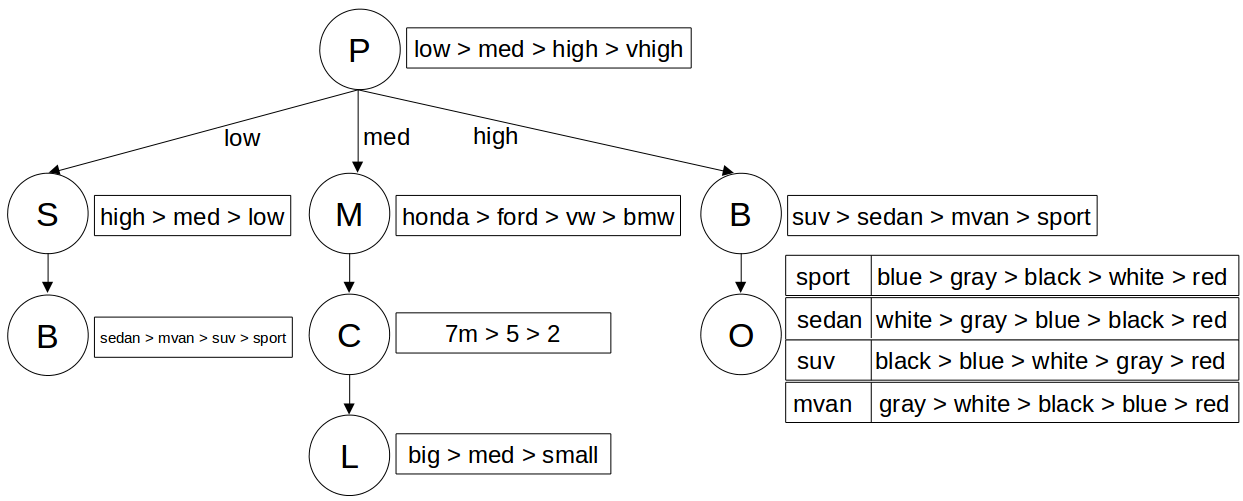
\includegraphics[width=0.9\textwidth]{figs/Cars/cicptree.png}
	  \caption{A CICP PLP-tree}
	\end{figure}

	According to this CICP PLP-tree, \tit{Car1} is preferred to \tit{Car2}.
}
